As previously mentioned, we measure research connectivity as the collaboration between authors across units within the same organization and across different institutions. The following graphs and tables are the results we produced from the sample size.

\begin{figure}[h]
  \centering
  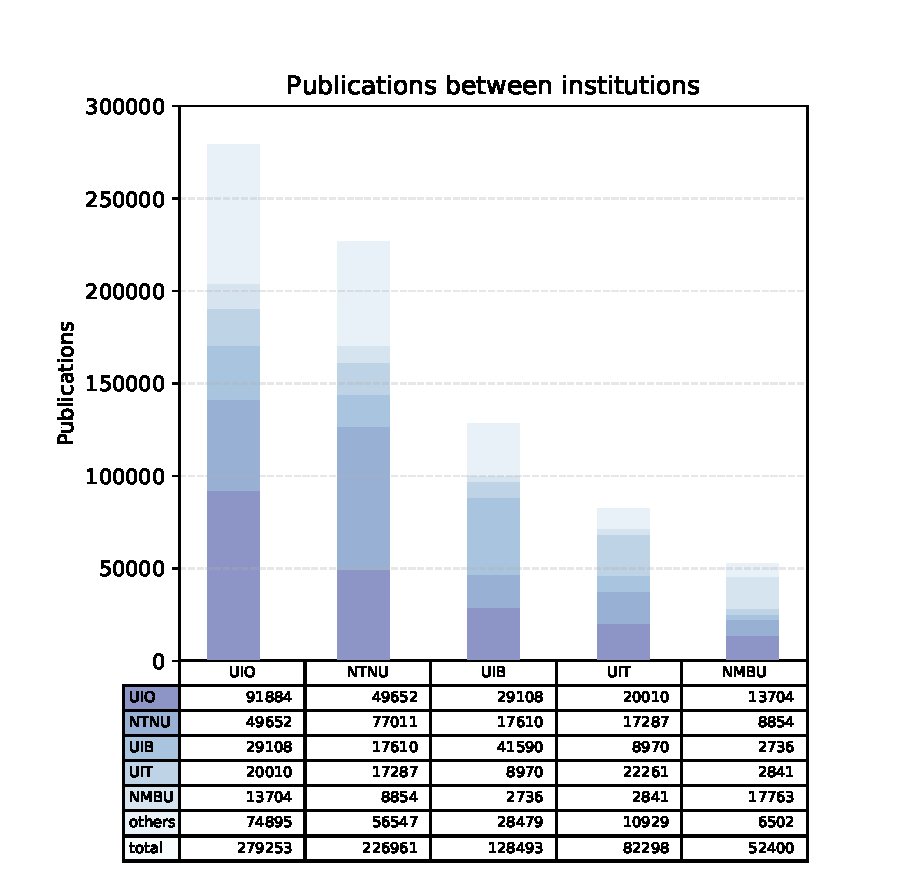
\includegraphics[width=0.5\textwidth]{table.pdf}
  \caption{Publications between institutions}
  \label{fig:result}
\end{figure}

\Fref{fig:result} shows UiO to be the institution with the greatest number of results, with NTNU following relatively close, and UiB, UiT and NMBU at much lower numbers.
An interesting observation is UiO’s cooperation with other institutions, among those, Oslo University Hospital, which they have a large number of joint results. Something that is not surprising.
Similarily, a large number of NTNU’s results are attributed to research in conjunction with UiO. This is expected as NTNU and UiO are the two largest institutions in Norway by far.


\begin{figure}[h]
	\centering
	\begin{tabular}{| l || c | c |}
		\hline
		Institution	& Only same institution	& Cross institution	\\ \hline
		UiO		& 0.329			& 0.671			\\
		NTNU		& 0.339			& 0.661			\\
		UIB		& 0.324			& 0.676			\\
		UiT		& 0.270			& 0.730			\\
		NMBU		& 0.339			& 0.661			\\
		\hline
	\end{tabular}
	\caption{Proportion of cross institution and only same institution results}
	\label{tab:institution-proportion}
\end{figure}

From \Fref{tab:institution-proportion}, we observe that all five institutions have more than $2/3$ of their results where the authors are employed at different institutions. UiT in particular is even higher than the other institutions, with close to 0.5 of it’s results being in coordination with either UiO or NTNU. As with UiT, NMBU has a large part of it’s results in conjunction with UiO, probably due to them being located relatively close to one another. Why then, UiT is so heavily influenced by the research at UiO and NTNU, is not known.

\begin{figure}[h]
	\centering
	\begin{tabular}{| l || c | c |}
		\hline
		Institution	& Only same unit	& Cross unit	\\ \hline
		UiO		& 0.226			& 0.774		\\
		NTNU		& 0.543			& 0.457		\\
		UIB		& 0.505			& 0.495		\\
		UiT		& 0.320			& 0.680		\\
		NMBU		& 0.661			& 0.339		\\
		\hline
	\end{tabular}
	\caption{Proportion of cross unit and only same unit results}
	\label{tab:unit-proportion}
\end{figure}

In \Fref{tab:unit-proportion}, we see that UiO is the institution who has the highest proportion of published results across units, surprisingly NTNU has the lowest proportion together with NMBU. An important observation is that UiO has 669 registered units against NTNUs 97 registered units and NMBUs 16 registered units, and as mentioned above NTNU and UiO are largest institutions in Norway. The reason for NTNUs and NMBUs low proportion of published results across units is that they have a higher rate of persons per units then institutions like UiT and UiO with a low rate of persons per units.
